
This paper develops the \rrtfunnel{} algorithm, by two means: First it employs
robust motion primitives generated by the the SOS programming framework based on
the work by \cite{majumdarFunnelLibrariesRealtime2017}, and second, deploy these
funnels as robust motion primitives in a discrete RRT robust motion planner
based on \cite{Lav06}. Using robust motion primitives has several advantages.
Firstly, they handle uncertainty, and thus, as long as the uncertainties in the
system are akin to the assumptions on the incoming uncertainty parameters, the
dynamical system will not leave the funnel, and hence if the funnel is not in
collision, neither will the system be. Secondly, as the motion primitives are
robust, there is no need for more conservative maneuvers and heuristics, such as
maximizing the distance to an obstacle, which is a naive way for motion planners
to handle uncertainty. Since the primitives are robust, the system might as well
choose a primitive that is close to an obstacle, as one that is far away, since
the funnel is guaranteed to be collision-free in both cases. This means that a
robust motion algorithm can perform more aggressive maneuvers than one that is
inherently conservative about its environment and
maneuvers~\cite{singhRobustOnlineMotion2017}.


\subsection{Generating Robust Motion Primitives}
\label{sec:generating-robust-motion-primitives}

\subsubsection{Generating Trajectories}
\label{subsec:generating-the-trajectories}

The robust motion primitives are \textit{finite regions of time variance} around
an initial trajectory, meaning that they are all the states surrounding a
trajectory in which the system can reach in a given time. But in order to verify
the robust regions surrounding a trajectory, first the trajectories themselves
have to be generated. Generating optimal trajectories is a rich field in the
motion planning literature~\cite{Betts_1998}. The initial trajectories can be
generated by many different methods, however the \textit{direct collocation
method} suited the needs of this paper best~\cite{von1993numerical}. It was
chosen as it builds locally optimal trajectories from a discrete set of sampled
points along a sought trajectory, which is beneficial for the discrete funnel
verification in \cref{subsec:generating-funnels}. For this problem the cost
function chosen for the solver to minimize is:
\begin{equation}
  J = \int_{0}^{T} \left[ 1 + {\vect{u}_{0}}^{T} \matr{R} \vect{u}_{0} \right] \mathrm{d}t,
\end{equation}
where \(\matr{R} = 1\), because it will minimize the system input, and thus give
a smooth output trajectory~\cite{majumdarRobustOnlineMotion2013}.

\subsubsection{Initializing the Funnel Calculations}
\label{subsec:initializing-tvlqr}

The funnel calculation algorithm has to be initialized with a candidate Lyapunov
function. In the same way as in Majumdar~\cite{majumdarRobustOnlineMotion2013},
the funnel generation algorithm will be initialized with a TV-LQR controller as
the initial Lyapunov function employing a cost function of the form
\begin{IEEEeqnarray*}{ll}
  J &= \vect{x}^{T} (t_f) \matr{F}(t_f) \vect{x} (t_f) \IEEEyesnumber \\
    &+ \int_{t_{0}}^{t_{f}} \left( \vect{x}^{T} \matr{Q} \vect{x} + \vect{u}^{T} \matr{R} \vect{u} + 2 \vect{x}^T \matr{N} \vect{u} \right) \mathrm{d}t,
\end{IEEEeqnarray*}


\subsection{Generating the Funnels around the Initial Trajectories}
\label{subsec:generating-funnels}

With the nominal trajectories, and the initial Lyapunov functions ready, the
funnels around the nominal trajectories can be calculated using
\cref{alg:funnelalgorithm} on page~\pageref{alg:funnelalgorithm}, and is
implemented in software through the \textsc{sostools}~\cite{sostools} toolbox.

However, the dynamics for the model in \cref{eq:model-dynamics-cl} are still not
polynomial, given the \(\sin\) and \(\cos\) terms
in~\eqref{eq:model-dynamics-cl}, and the SOS-framework can only verify
polynomial systems. Thus in order to obtain the needed polynomial dynamics, the
system is expanded around the nominal trajectory with a Taylor expansion of
degree three. The function limiting the size of the funnel \(\rho(t_{k})\) also
has to be initialized by a feasible upper bound \(\rho(t)\). This is done
through the equation
\begin{equation}
  \rho(t_{k}) = \mathrm{exp}\left( \rho_{\tau}\frac{\left( t_{f} - t \right)}{\left( t_{f} - t_{0}  \right)}\right) + \rho_0
\end{equation}
where \(\rho_{\tau}\) is a positive constant determining the upper bound on the
funnel, along with the zero value \(\rho_0\). If the given choice of
\(\rho_{\tau}\) does not verify a funnel, either increase the value of
\(\rho_{\tau}\) and \(\rho_0\), and optionally the number of sampled points from
the trajectory to be verified~\cite{Tobenkin_2011}.

The initial condition set also has to be decided before the reachable set can be
calculated. In general the initial condition set can be any semi-algebraic set
in the state-space. However, a simple way of obtaining an initial condition set
for the trajectories at hand is by taking advantage of the Lyapunov function
candidate from the LQR-controller~\cite{tedrakeLQRtreesFeedbackMotion2009}.
Thus by setting
\begin{equation}
  \mathcal{X}_{0} = \frac{ \matr{S}_{k}}{\rho_{\tau}},
\end{equation}
an initial condition set is obtained. In general however, any semi-algebraic set
will do, and the algorithm is not constrained to this one initial condition set
in particular, but it has proven itself useful when calculating new motion
primitives for a system when the initial condition set is not obvious. Another
idea is to use the outlet of one funnel as the initial condition set for the
calculation of the next.

\subsection{Funnel Transformations and Invariance}
\label{subsec:shifting-funnels}

Now that the funnels are able to be calculated for a basic set of motion
primitives, it is time to start looking at chaining these primitives together in
order to construct longer and more complex motions from a basis of motion
primitives. Thus, in order to freely shift funnels around in the configuration
space, the cyclic coordinates of the system have to be determined, so that the
dynamics of the system is never violated. Even though the funnels can now start
and end in a completely different part of the configuration space, the original
dynamics must not be violated. Therefore the cyclic and non-cyclic coordinates
of the system must be decided.



\subsection{Sequential Funnel Composition}
\label{sec:composable-funnels}

Since the funnels can be shifted freely around the configuration space along the
cyclic coordinates of the system to create new motion primitives, the funnels
can now be composed together by the RRT algorithm into the planning environment
in and create a guaranteed robust motion plan.

However, in order for two funnels to create a third and new motion primitive
when chained together, they need to be composable. This means that the inlet of
the second funnel needs to be fully contained within the outlet of the first
one. Otherwise the robustness guarantees of the traversal will be lost. An
abstract pictorial representation of two funnels composed together can be seen
in~\cref{fig:two-funnels-composed} to emphasize this observation.

The mathematical definition of funnel composition
(\cref{def:funnel-composition}) that is used to verify that two funnels are
composable is not in accordance with the new transformed funnels from
\cref{subsec:shifting-funnels}. However, take note that the definition only has
to be modified slightly in order to take into account the translation along the
cyclic coordinates of the system.
\begin{definition}
  \label{def:invarant-funnel-composition}
  An ordered pair \((F_1,F_2)\) of funnels \(F_1 \colon [0,T_1] \rightarrow
  \mathcal{P}(\R^n)\) and \(F_2 \colon [0,T_2] \rightarrow \mathcal{P}(\R^n)\)
  is \textit{sequentially composable modulo invariance} if there exists a shift
  along cyclic coordinates such that \(F_{1}(T_1) \subset
  \Psi_{c}\bigl(F_2(0)\bigr) \).
\end{definition}
In layman's terms this means that if a funnel \(F_2\) can be shifted along
cyclic coordinates to stack up against the outlet of funnel \(F_2\) so that they
are composable in the sense of \cref{def:funnel-composition}, they are
composable modulo
invariance~\cite[definition~3,sec~5]{majumdarFunnelLibrariesRealtime2017}. Since
any funnel in the configuration space will be a set consisting of the funnel
from the basic set, along with a transformation along the cyclic coordinates of
the system, the set of all funnels, \(\hat{\mathcal{F}}\), in the configuration
space, is written \(\hat{\mathcal{F}} = \set{F_n \in \R^n \mid \Psi_{c,i}(F_i),
  F_i \in \mathcal{F}}\). Here \(\mathcal{F}\) is the basic set of funnels, and
since the transformation is already known the composability is straightforward
to compute.

\begin{figure}[!t]
  \centering {
\includegraphics[width=.8\columnwidth]{figures/method/funnel-composition}}
  \caption[Two composable funnels]{Two funnels that can be successfully composed, as the outlet of the
    first one is fully contained in the inlet of the second.}
  \label{fig:two-funnels-composed}
\end{figure}

Therefore apply the generalized S-procedure on
\begin{equation}
  V_1(T_1,\bar{\vect{x}}) \leq \rho_1(T_1) \implies V_2(0, \bar{\vect{x}}) \leq \rho_2(0) \mathEoS
\end{equation}
Then the composability of two funnels can be checked through the SOS program
\begin{IEEEeqnarray*}{ll}
   \text{Find } L(\vect{x}) \IEEEyesnumber \\
  \text{s.t.} \\
   \IEEEeqnarraymulticol{2}{r}{\rho_2(0) - V_2(0,\vect{x}) - L(\vect{x})\left( \rho_1(T_1) - V_1(T_1,\vect{x}) \right) \text{ is SOS}} \\
  \IEEEeqnarraymulticol{2}{r}{L(\vect{x}) \text{ is SOS}} \mathEoS
\end{IEEEeqnarray*}
Which is implemented using \textsc{sostools}~\cite{sostools} and \matlab{}.


\subsection{Invariance of the Funnels Calculated}

The funnels generated are \textit{outer approximations} of reachable sets for
the system at hand~\cite{majumdarFunnelLibrariesRealtime2017}. This means that
in general they are larger than the actual reachable set for the system. This
can be verified through a Monte-Carlo simulation. Running N-simulations from the
funnel inlet, and storing the solutions, it is possible to visualize the actual
funnel for the system. 

By comparing one of the funnels in the funnel set with a funnel based from
\(10.000\) simulation runs, it is seen that the calculated funnels are indeed
proper outer approximations of the time-reachable sets for the uncertain
dynamical system. Therefore, the conclusion is that the uncertain trajectories
are contained within the funnels used in the planner, and the trajectories can
be seen as robust to uncertainty given the uncertainty and dynamical assumptions
made.

\section{RRT}
\label{sec:RRT}

With the basic framework for dealing with funnels as motion primitives
constructed, it is time to build the RRT part of the \rrtfunnel{} algorithm. The
reason for basing the global path planning framework on the RRT motion planning
algorithm is as follows. One, it has the ability to quickly expand deep into the
search-space, and then later progress towards a finer sampling, which is
valuable as it avoids local minima. Two, the RRT algorithm is easily extensible
to larger state spaces, and thus adding to the generality of the \rrtfunnel{}
algorithm, such that it can be adapted to fit a wide range of dynamical systems,
while at the same time it has only three main components that needs to be in
place in order for successful path planning to succeed in an arbitrary
configuration space. Namely, a suitable probability distribution to sample from,
and a distance metric for the nearest neighbor and the extension step. The RRT
algorithm is beneficial as most of the complexity accompanied with the planning
problem (like uncertainty and controller calculations) has already been handled
by the SOS framework, and hence the RRT algorithm need only concern itself with
stacking one robust motion primitive after the other without any concern for the
complexities mentioned above.

\subsection{Distance in Configuration Space}

The \rrtfunnel{} algorithm will use the same metric for both the closest node
and the extend operation on the funnel graph. The metric chosen is a modified
Euclidean metric which weights the angle \(\theta\) depending on how close the
airplane is to the final configuration, and is defined as
\[
  \rho(\vect{x}_{1}, \vect{x}_{2}) = w_{1}\norm{\mathnormal{X_{1}} -
    \mathnormal{X_{2}}} + w_{2}f(\theta_1,\theta_2) ,
\]
where \(\norm{\mathnormal{X_{1}} - \mathnormal{X_{2}}}\) is the standard
Euclidean metric, \(f\) is a function giving the distance between
headings~\cite{kuffnerEffectiveSamplingDistance2004}. The rotations and distance
is then scaled relative to the translation distance. Which helps solve some of
the problems with the Euclidean distance metric \cite{lav06}.

\subsection{The Funnel-Graph}

Even though the \rrtfunnel{} algorithm can work just fine with a collection of
funnels, and simply brute-force all funnels at the planning stage, it is helpful
to associate some kind of structure with the collection. Therefore the funnels
will be organized into a graph structure \(\mathcal{G}\) where each funnel is an
edge in the graph, and the inlets and the outlets are vertices. The planner
needs information about which funnels that are composable, as they may not all
be composable with each other, implying that the resultant graph is not
necessarily complete.

\begin{figure}[!t]
  \begin{minipage}[l]{.45\columnwidth}
    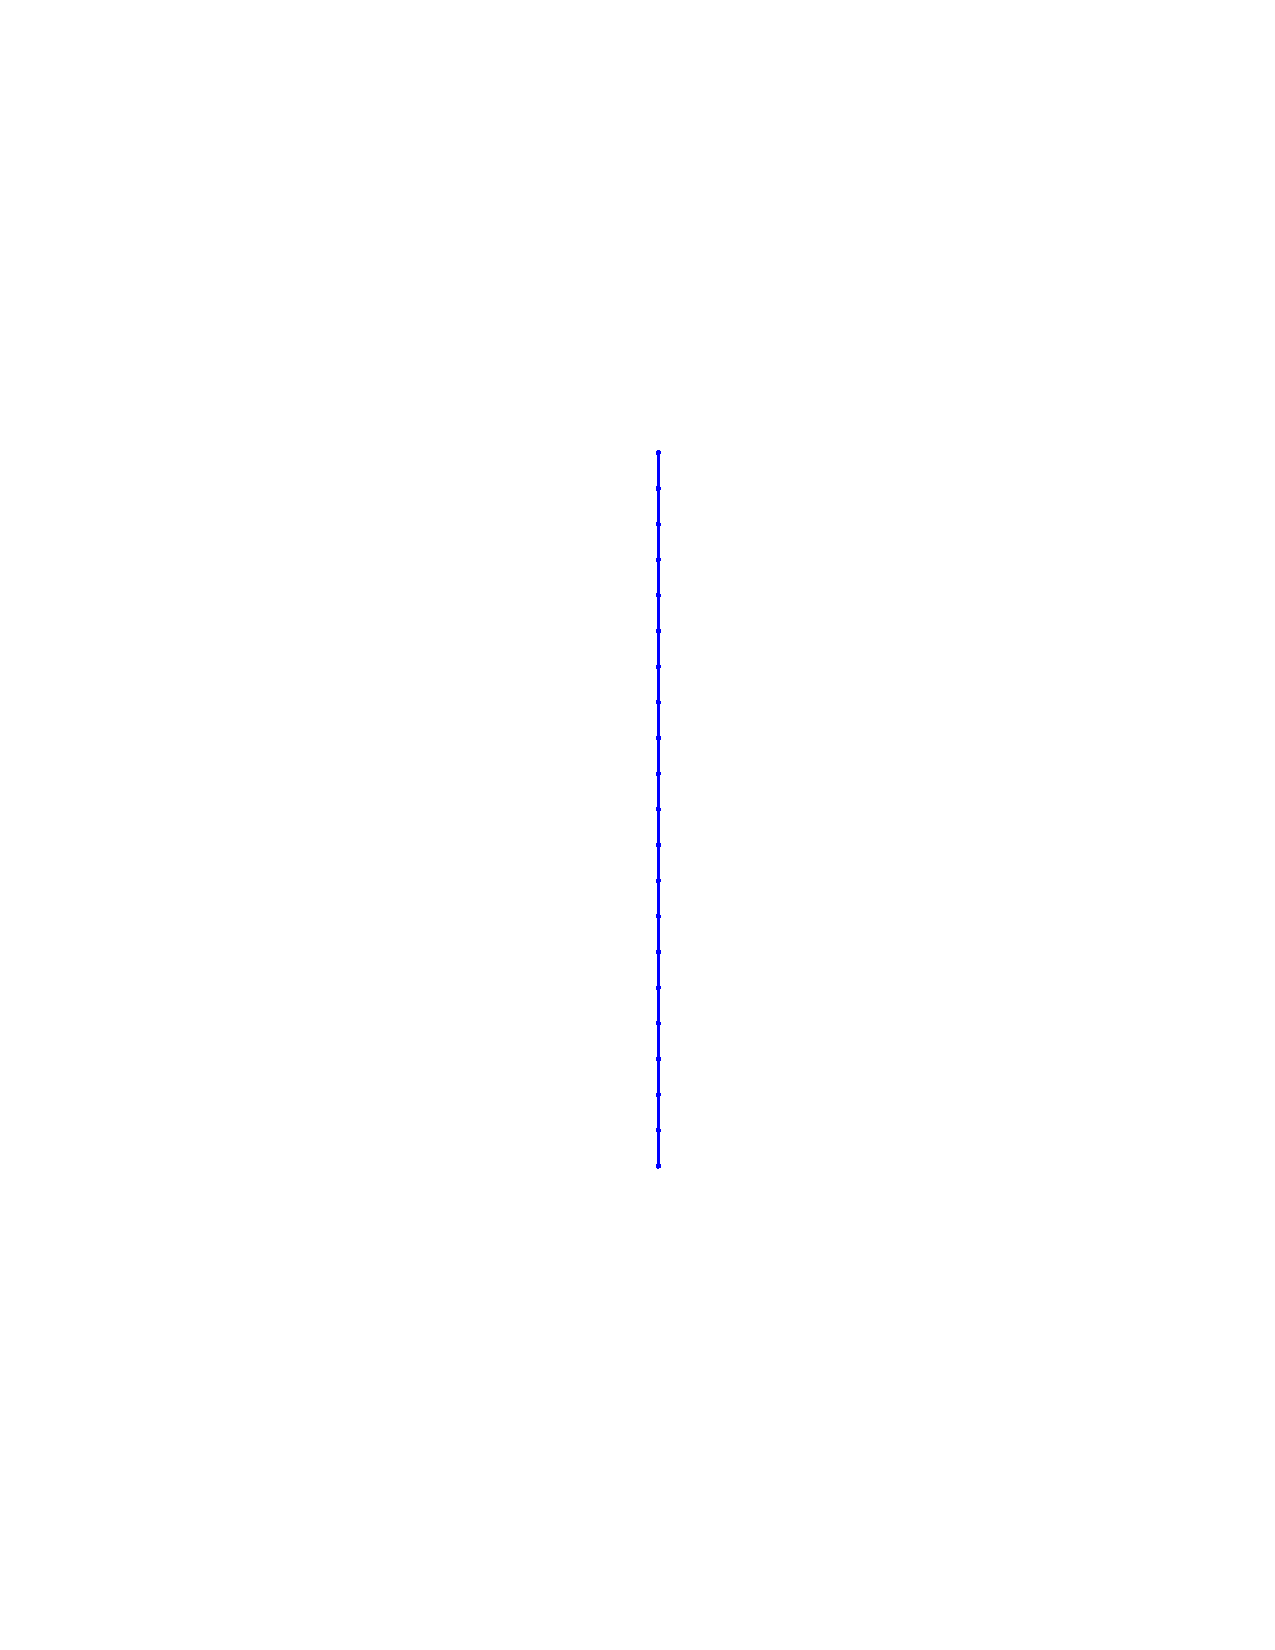
\includegraphics[trim={-5cm 5cm -5cm 5cm},
    width=.9\columnwidth,
    scale=20]
    {figures/method/trajectory-sampled}
    \caption{Trajectory sampled 21 times.}
  \end{minipage} \; %
  \begin{minipage}[r]{.45\columnwidth}
    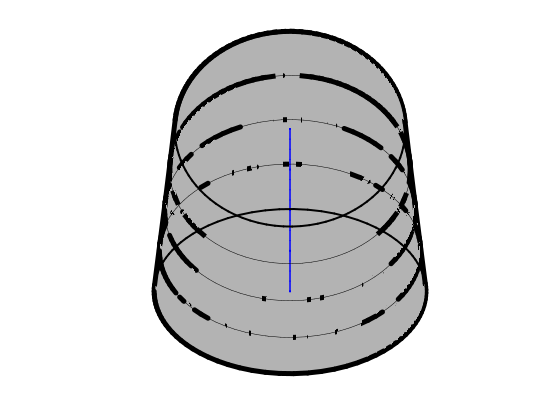
\includegraphics[trim={-5cm 5cm -5cm 5cm},
    width=.9\columnwidth,
    scale=20]{figures/method/funnel-sampled}
    \caption{The verified trajectory ellipsis overlaid at the sample times.}
    \label{fig:funnel-straight-sampled}
  \end{minipage}
\end{figure}


\subsection{Expanding the Size of the Funnels}

In general the funnels generated are computed for the point model in
\cref{eq:dynamicalsystem} only, and hence, in order to run the algorithm with a
model of some size, the funnels have to be expanded by the largest radius of the
given model. As the funnels are ellipsis around the point at the trajectory that
they verify, the funnels can be expanded by any radius with a linear
transformation. An expansion of the point model funnel can be seen in
\cref{fig:expanded-funnel}.


\begin{figure}[!t]
  \centering 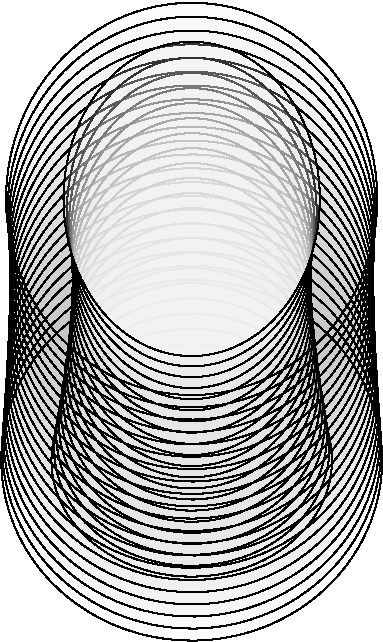
\includegraphics[scale=.3]{figures/method/expanded-funnel}
  \caption[The expanded experiment funnel]{The original funnel created from the point model, with a funnel
    expanded by a radius of 0.1 surrounding it.}
  \label{fig:expanded-funnel}
\end{figure}
